\chapter{Bifurcations of fixed points}
\section{Local nonlinear dynamics near fixed points}
We are interested in the local nonlinear dynamics around fixed points. Consider
\begin{align}
	\dot{x}=f(x);\quad f\in C^{r},r \geq 1; \quad f(p) = 0, \numberthis \label{eq:4star}
\end{align}
i.e. $p$ is a fixed point of the dynamical system. The linearized system at $p$ is
\begin{align}
	\dot{y} = Df(p)y,\ y\in \mathbb{R}^{n},\ Df(p)\in \mathbb{R}^{n \times n}. \numberthis \label{eq:4sstar}
\end{align}
The linearization has the eigenvalues $\lambda_1, \ldots, \lambda_n \in \mathbb{C}$ with multiplicities counted. Corresponding to these eigenvalues are the eigenvectors $e_1,\ldots,e_n \in \mathbb{C}^{n}$, including generalized eigenvectors for when the algebraic multiplicity is greater than the geometric multiplicity. The eigenvector $e_j$ is real when $\lambda_j \in \mathbb{R}$.

\begin{definition}
The following subspaces are invariant for the linearized dynamical system:
\begin{enumerate}
	\item The \emph{stable subspace}
		\begin{align}
			\boxed{
				E^{S} =  \textrm{span} _{j}\left \{  \textrm{Re} (e_j),  \textrm{Im} (e_j):\  \textrm{Re} (e_j) < 0\right\},
			}
		\end{align}
	\item The \emph{unstable subspace}
		\begin{align}
			\boxed{
				E^{U} =  \textrm{span} _{j}\left \{  \textrm{Re} (e_j),  \textrm{Im} (e_j):\  \textrm{Re} (e_j) > 0\right\},
			}
		\end{align}
	\item The \emph{center subspace}
		\begin{align}
			\boxed{
				E^{C} =  \textrm{span} _{j}\left \{  \textrm{Re} (e_j),  \textrm{Im} (e_j):\  \textrm{Re} (e_j) = 0\right\}.
			}
		\end{align}
\end{enumerate}

\end{definition}
\begin{remark}[]
	Note here that the following facts hold
	\begin{enumerate}
		\item $E^{C}= \emptyset$ if and only if $p$ is hyperbolic,
		\item $E^{U,S}$ and $E^{C}$ are invariant subspaces of \eqref{eq:4sstar} by construction,
		\item Solutions of \eqref{eq:4sstar} in $E^{S}$ (resp. $E^{U}$) decay to $y=0$ as $t \to \infty$ (resp. $t \to - \infty$). 
	\end{enumerate}
	
\end{remark}

We now ask ourselves what happens to these subspaces in the nonlinear system.
\begin{theorem}[Center Manifold Theorem]
	The following hold:
	\begin{enumerate}
		\item There exists a unique \emph{stable manifold} $W^{S}(p)$ for \eqref{eq:4star}, such that
	\begin{itemize}
		\item $W^{S}(p)$ is a $C^{r}$ manifold (surface), tangent to $E^{S}$ at $p$ with $ \textrm{dim} W^{S}(p) =  \textrm{dim} E^{S}$,
		\item $W^{S}(p)$ is invariant for \eqref{eq:4star} and for $x\in W^{S}(p)$ we have 
			\begin{align}
				\| F^{t}(x) \| \leq K_{S} \exp\left[ t \left( \max_{ \textrm{Re} (\lambda_j) < 0}( \textrm{Re} (\lambda_j)) + \epsilon_S \right) \right]
			\end{align}
	 for $t\geq 0$, $0 < \epsilon_S \ll 1$, and  $\| x- p\|$ small enough.
	\end{itemize}
			
		\item There exists a unique \emph{unstable manifold} $W^{U}(p)$ for \eqref{eq:4star}, such that
	\begin{itemize}
		\item $W^{U}(p)$ is a $C^{r}$ manifold (surface), tangent to $E^{U}$ at $p$ with $ \textrm{dim} W^{U}(p) =  \textrm{dim} E^{U}$,
		\item $W^{U}(p)$ is invariant for \eqref{eq:4star} and for $x\in W^{U}(p)$ we have 
			\begin{align}
				\| F^{t}(x) \| \leq K_{U} \exp\left[ t \left( \max_{ \textrm{Re} (\lambda_j) > 0}( \textrm{Re} (\lambda_j)) + \epsilon_U \right) \right]
			\end{align}
	 for $t\geq 0$, $0 < \epsilon_U \ll 1$, and  $\| x- p\|$ small enough.
	\end{itemize}
			
\item There exists a (not necessarily unique) \emph{center manifold} $W^{C}(p)$ for \eqref{eq:4star}, such that
	\begin{itemize}
		\item $W^{C}(p)$ is a $C^{r-1}$ manifold (surface), tangent to $E^{C}$ at $p$ with $ \textrm{dim} W^{C}(p) =  \textrm{dim} E^{C}$,
	\end{itemize}
			
	\end{enumerate}
	
\end{theorem}
The geometry of these manifolds is sketched in Fig. \ref{fig:mfds_def}.
\begin{figure}[h!]
	\centering
	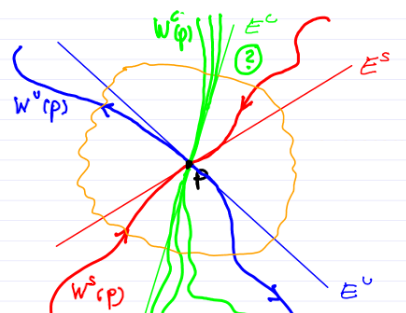
\includegraphics[width=0.6\textwidth]{figures/ch3/1manifolds_def.png}
	\caption{A sketch of the stable (red), unstable (blue), and center manifolds (green), along with their respective invariant linear subspaces. Note the existence of multiple center manifolds and the singular unique unstable/stable manifolds.}
	\label{fig:mfds_def}
\end{figure}

The overall dynamics depend crucially on the center manifold, especially when $E^{U}= \emptyset$, i.e. the stability type is determined by $W^{C}(p)$. Hence why it will be the subject of our further investigation.

\section{The center manifold}
\begin{ex}[Uniqueness of the center manifold]
	We would like to explore if the center manifold is generally non-unique. Consider the dynamical system
	\begin{align}
\begin{dcases}
	\dot{x} = x^2 \\
	\dot{y} = -y.
\end{dcases}
	\end{align}
	First, linearize at the origin to find the linearized dynamics
	\begin{align}
		A = Df(0) = 
		\begin{pmatrix}
			0 & 0 \\ 0 & -1
		\end{pmatrix}
		.
	\end{align}
	These linearized dynamics are illustrated in Fig. \ref{fig:cmfd_lin_ex}. We find the invariant subspaces
	\begin{align}
		E^{C} =  \textrm{span}\left\{ 
			\begin{pmatrix}
				1 \\ 0 
			\end{pmatrix}
		\right\};\quad
		E^{S} =  \textrm{span}  \left\{
			\begin{pmatrix}
				0 \\ 1
			\end{pmatrix}
		\right\}; \quad
		E^{U} = \emptyset.
	\end{align}
	The nonlinear manifolds are illustrated with the invariant subspaces from the linearization in Fig. \ref{fig:cmfd_lin_ex}.
	\begin{figure}[h!]
		\centering
		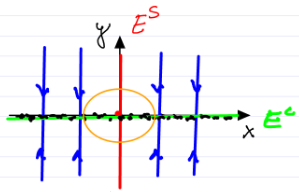
\includegraphics[width=0.45\textwidth]{figures/ch3/2cmfd_lin_ex.png}
		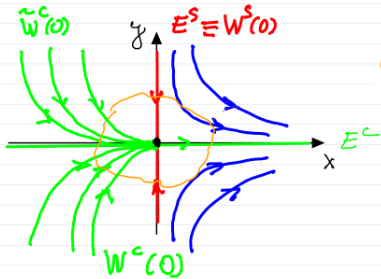
\includegraphics[width=0.4\textwidth]{figures/ch3/3cmfd_nonlin_ex.png}
		\caption{Left: The linearized dynamics around the origin. Right: The nonlinear phase portrait. }
		\label{fig:cmfd_lin_ex}
	\end{figure}
	Observe there exist infinitely many center manifolds which are all invariant and all tangent to $E^{C}$ at the origin. We also see that although the fixed point at the origin is stable in the linearized system, it is unstable in the nonlinear system.
\end{ex}

We are left with the question: how can we calculate $W^{C}(p)$ in general? 
\begin{enumerate}
	\item Consider 
		\begin{align}
			\dot{z} = F(z); \quad F(0) = 0;\quad z \in \mathbb{R}^{c+d};\quad F \in C^{r}.
		\end{align}
		Where $c$ represents the number of center directions at the origin ($ \textrm{dim}E^{C}$) and $d$ denoted the remaining directions ($ \textrm{dim} E^{U} +  \textrm{dim} E^{S}$).
	\item Now block-diagonalize the linearization. This consists of four steps
		\begin{enumerate}
			\item First linearize the dynamics to find $\dot{z} = Mz + \mathcal{O}(\|z\|^2)$ with $M = DF(0) \in \mathbb{R}^{(c+d) \times (c+d)}$.
			\item Define the transformation matrix
				\begin{align}
					T=
					\begin{bmatrix}
						a_1 & \ldots & a_c & b_1 & \ldots & b_d	
					\end{bmatrix}
				=
				\begin{bmatrix}
					\textrm{basis in } E^{C} &  \textrm{basis in } E^{U} \oplus E^{S}
				\end{bmatrix}
				.
				\end{align}
			\item Pass to the basis from the transformation matrix with $z = T \xi$
				\begin{align}
					\dot{\xi} = T^{-1}\dot{z} = T^{-1}MT \xi + T^{-1}\mathcal{O}(\| T\xi\|^2) = 
					\begin{pmatrix}
						A & 0 \\
						0 & B
					\end{pmatrix}
					\xi + \mathcal{O}(\| \xi \| ^2).
				\end{align}
			The matrices $A$ and $B$ are elements of $\mathbb{R}^{c \times c}$ and $\mathbb{R}^{d \times d}$ respectively.	
		\item Let $\xi = 
			\begin{pmatrix}
				x \\ y
			\end{pmatrix}
			\in \mathbb{R}^{c}\times \mathbb{R}^{d}$, the $x$-coordinates is aligned with $E^{C}$ and the $y$-coordinates are perpendicular. We then find
			\begin{align}
				\dot{x} = Ax + f(x,y);\quad \dot{y} = By + g(x,y),
			\end{align}
			for $f,g \in C^{r}$ and $f,g = \mathcal{O}(\|x\|^2, \|y\|^2, \|x\|\|y\|)$. The geometry in these coordinates is depicted in Fig. \ref{fig:cmfd_trafo_geom}. The center manifold is given by
			\begin{align}
				W^{C}(0) = \left\{ (x,y) \in U:\ y = h(x)\right\}
			\end{align}
			for $h:\mathbb{R}^{c} \to \mathbb{R}^{d}$ and $ h \in C^{r-1}$ as in the theorem.
			\begin{figure}[h!]
				\centering
				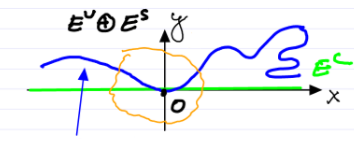
\includegraphics[width=0.4\textwidth]{figures/ch3/4cmfd_trafo_geom.png}
				\caption{The geometry of the nonlinear system in the transformed coordinates aligned with the invariant subspaces of the linearization. The blue arrow points to the center manifold $W^{C}(0)$.}
				\label{fig:cmfd_trafo_geom}
			\end{figure}
		\end{enumerate}
	\item Now we use the invariance of $W^{C}(0)$, i.e. for all $t$ it holds $y(t) = h(x(t))$ to find
		\begin{align}
			\dot{y} = Dh(x(t)) \dot{x}(t),
		\end{align}
		which implies the nonlinear partial differential equation (PDE) for $h(x)$
\begin{align}
	\boxed{
		Bh(x) + g(x, h(x)) = Dh(x) \left[ Ax + f(x, h(x))\right] \numberthis \label{eq4:1star}.
	}
\end{align}
We cannot solve this analytically.
\item Instead take the Taylor expansion of \eqref{eq4:1star} to approximate the solution
	\begin{align}
		h(x) = \underbrace{h(0)}_{=0} + \underbrace{Dh(0)}_{=0}x + \frac{1}{2} \underbrace{D^2h(0)}_{3- \textrm{tensor} } \otimes x \otimes x + \mathcal{O}(\|x \| ^3),
	\end{align}
	where the first two terms are 0 due to the tangency to $E^{C}$ at $0$. We therefore have that $h(x) = \mathcal{O}(\|x\|^2)$. Therefore we seek $W^{C}(0)$ of this form. We get the dynamics on the center manifolds 
	\begin{align}
		\boxed{
			\dot{x}=Ax+f(x,h(x)).
		}
	\end{align}
\end{enumerate}

\begin{ex}[Finding the center manifold]
	Consider the dynamical system
	\begin{align}
		\begin{dcases}
			\dot{x}=xy \\
			\dot{y}=-y+\alpha x.
		\end{dcases}	
	\end{align}
	First we linearize at $(0,0)$ to get 
	\begin{align}
		M =
		\begin{pmatrix}
			[0] & [0] \\
			[0] & [-1]
		\end{pmatrix}
	\end{align}
	which is already in block-matrix form. The dimensions of the stable, unstable, and center subspaces of the linearization are 1, 0, and 1 respectively. Hence the stability type depends on the dynamics on the center manifold $W^{C}(0)$. We now look for an equation to parameterize $W^{C}(0)$
	\begin{align}
		h(x) = ax^2 + bx^3 + cx^4 + \mathcal{O}(x^5).
	\end{align}
	This is a finite expansion and thus in general will not converge as that would imply the center manifold is unique. Now use the invariance (the PDE we already derived) to find
	\begin{align}
		\dot{y} = h'(x)\dot{x} = \left[2ax+3bx^2 + 4cx^3 + \mathcal{O}(x^4) \right] x \left[ax^2+bx^3+cx^4 + \mathcal{O}(x^5) \right]. \numberthis \label{eq4:one}	
	\end{align}
	On the other hand, from the dynamical system we know
	\begin{align}
		\dot{y}=-h(x) + \alpha x^2 =(\alpha - a) x^2 -bx^3 - cx^4 + \mathcal{O}(x^5). \numberthis \label{eq4:two}
	\end{align}
	Comparing coefficients of equal powers in \eqref{eq4:one} and \eqref{eq4:two}.
	\begin{align}
		\mathcal{O}(x^2)&:\ \alpha = a\\
		\mathcal{O}(x^3)&:\ b=0 \\
		\mathcal{O}(x^4)&:\ 2a^2 = -c.
	\end{align}
	Therefore we find 
	\begin{align}
		\boxed{
	h(x) =\alpha x^2 - 2\alpha^2x^4 + \mathcal{O}(x^5).}
	\end{align}
	Then the dynamics on $W^{C}(0)$ become
	\begin{align}
		\boxed{
			\dot{x}= xh(x) = \alpha x^3(1-2\alpha x^2) + \mathcal{O}(x^6). \numberthis \label{eq4:2star}
		}
	\end{align}
	These dynamics are depicted in Fig. \ref{fig:cmfd_alpha_diff}. For $\alpha > 0$ the origin is unstable, meanwhile for $ \alpha <0$ the origin is asymptotically stable.
	\begin{figure}[h!]
		\centering
		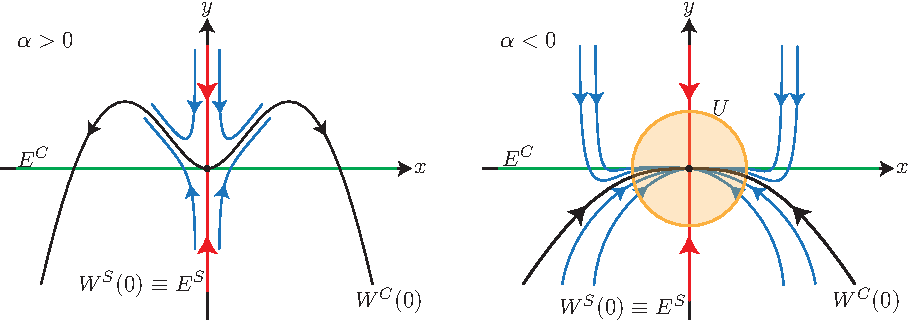
\includegraphics[width=0.8\textwidth]{figures/ch3/5cmfd_alpha_diff}
		\caption{Left: The nonlinear dynamics on the center manifold for $\alpha > 0$. Right: The nonlinear dynamics on the center manifold for $\alpha < 0$.}
		\label{fig:cmfd_alpha_diff}
	\end{figure}
	
	The full local stable manifold for $\alpha <0$ is $\overline{W}^{S}(0)=U$ and it is of dimension 2. The difference between $\overline{W}^{S}(0)$ and $W^{S}(0)$ is that in general the decay rate is generally weaker than the rate guaranteed in the Center Manifold Theorem. 

\begin{remark}[]
	The $\mathcal{O}(x^5)$ truncation has two hyperbolic fixed points at $x = \pm \frac{1}{\sqrt{2 \alpha} }$, however the full system has no such fixed points. The reason for this is that away from the origin, the $\mathcal{O}(x^6)$ terms are no longer guaranteed to be small relative to the $\mathcal{O}(x^5)$ terms, and the truncation this far away from 0 is not justified.
\end{remark}
\end{ex}

After this example we would like to explore if the concept of the center manifold is robust, as the existence of eigenvalues with $ \textrm{Re} (\lambda_i) = 0$ is not. We will explore this in an example.

\begin{ex}[Perturbing the previous example]
	Consider the following perturbed dynamical system
	\begin{align}
		\begin{dcases}
			\dot{x} = xy + \epsilon x \\
			\dot{y} = -y + \alpha x^2
		\end{dcases}
;\quad |\epsilon | \ll 1.
	\end{align}
The linearization of this system yields
\begin{align}
	\begin{dcases}
		\dot{x} = \varepsilon x \\
		\dot{y} = -y.
	\end{dcases}
\end{align}
{\color{blue} I used varepsilon instead of epsilon here, I like that and think we should use it everywhere.}
Now the center manifold disappears as the center subspace $E^{C}$ disappears for $\epsilon>0$!
\end{ex}

\section{Center manifolds depending on parameters}
We begin with the setup
\begin{align}
	\begin{dcases}
		\dot{x} = Ax + f(x,y,\epsilon) \\
		\dot{y} = By + g(x,y,\epsilon)
	\end{dcases}
;\quad x \in \mathbb{R}^{c},\ y \in \mathbb{R}^{d},\ 0\leq \epsilon \ll 1;\\
f,g \in C^{r},\ f,g=\mathcal{O}(\|x\|^2, \|y\|^2, \|x\|\|x\|, {\epsilon \|x\|, \epsilon \|y\|} ).
\end{align}
The order $\epsilon \|x\|$ and $\epsilon \|y\|$ terms are due to the perturbation of the linear part. Now assume $ \textrm{Re} (\lambda _j(A))= $ for $j=1,\ldots,c$ (the center directions) and $ \textrm{Re} (\lambda _j(B)) \neq  $ for $j=1,\ldots, $ (the hyperbolic directions). Next, rewrite $\tilde{x}=
\begin{pmatrix}
	x \\ \epsilon
\end{pmatrix}
$ and $\tilde{y}=y$ to obtain the system
\begin{align}
	\begin{dcases}
		\dot{\tilde{x}} = \tilde{A}\tilde{x} + \tilde{f}(\tilde{x}, \tilde{y}) \\
		\dot{\tilde{y}} = \tilde{B}\tilde{y} + \tilde{g}(\tilde{x}, \tilde{y}) 
	\end{dcases}
	;\quad \tilde{A}=
	\begin{pmatrix}
		A & 0 \\ 0 & 0	
	\end{pmatrix}
	\in \mathbb{R}^{(c+1)\times (c+1)}; \quad \tilde{f} =
	\begin{pmatrix}
		f \\ 0
	\end{pmatrix}. \numberthis \label{eq4:unostar}
\end{align}
Here, $\tilde{g}=g$ and $\tilde{B}=B$. Further, note that $ \textrm{span} \left\{
	\begin{pmatrix}
		x \\0
	\end{pmatrix}
\right\}$ is an invariant subspace for $\tilde{A}$. The eigenvalues of $\tilde{A}$ are the same as those of $A$ and an additional $0$, thus there are $c+1$ center directions and $d$ hyperbolic directions. Applying the center manifold theorem to the fixed point $0 \in \mathbb{R}^{c+1+d}$ of \eqref{eq4:unostar} we obtain that there exists a $\tilde{W}^{C}(0)$ $C^{r-1}$ manifold tangent to $E^{C}$ at $
\begin{pmatrix}
	\tilde{x} \\ \tilde{y}
\end{pmatrix}
= 
\begin{pmatrix}
	0 \\ 0
\end{pmatrix}
$ which is invariant and is dimension $c+1$. The geometry of this manifold is illustrated in Fig. \ref{fig:pert_cent_mfd}. Note in the figure that there is no dynamics in the $\epsilon$ direction, as $\dot{\epsilon}=0$ and that $(x,y)=(0,0)\in \mathbb{R}^{c+d}$ remains a fixed point for $\epsilon\neq 0$.
\begin{figure}[h!]
	\centering
	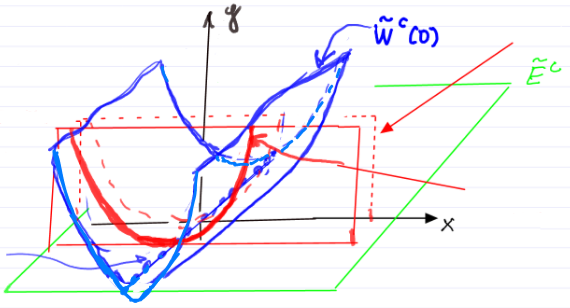
\includegraphics[width=0.7\textwidth]{figures/ch3/6pert_cent_mfd.png}
	\caption{Geometry of the center manifold with the perturbation. The straight red arrow designates the cut at $\epsilon=0$ which is equal to $W^{C}(0)$, the squiggly red arrow points at the continuation of the center manifold from $\epsilon=0$ to $\epsilon \neq 0$.}
	\label{fig:pert_cent_mfd}
\end{figure}

Computing $\tilde{W}^{C}(0)$ is done in a similar fashion as before. We use the center manifold theorem to get	
\begin{align}
	\tilde{y} = y= \tilde{h}(\tilde{x}) = \tilde{h}(x,\epsilon) = \mathcal{O}(\|x\|^2, \epsilon \|x\|, \epsilon^2) = \mathcal{O}(\|x\|^2, \epsilon \|x\|).
\end{align}
The order $\epsilon^2$ term was dropped as $x=0$ must remain a fixed point. The function $h$ describes the graph of $W^{C}_{\epsilon}(0)$. Then the reduced dynamics on $W^{C}_{\epsilon}(0)$ are
\begin{align}
	\boxed{
		\dot{x} = Ax + f(x, \tilde{h}(x, \epsilon), \epsilon).
}
\end{align}
This can then be applied to the perturbed example from above.

\begin{ex}[Revisting the perturbation]
	Recall the dynamical system
	\begin{align}
		\begin{dcases}
			\dot{x} = xy + \epsilon x\\
			\dot{y} = -y + \alpha x^2.
		\end{dcases}
	\end{align}
	We have the persisting fixed point at $(x,y)=(0,0)\in \mathbb{R}^{c+d}$	and the system is already in standard form with 
	 \begin{align}
		 A=0;\quad B=-1;\quad f(x,y,\epsilon) = xy + \epsilon x;\quad g(x,y,\epsilon) = -\alpha x^2.
	\end{align}
	We apply the center manifold theorem and get the existence of $W^{C}_{\epsilon}(0)$ for $|\epsilon|\ll 1$. This manifold satisfies
	 \begin{align}
		 y = \tilde{h}(x,\epsilon) = ax^2 + bx\epsilon + c\epsilon^2
		 +dx^3 + ex^2 \epsilon +j x\epsilon^2 + k\epsilon ^3
		 +kx^4. \ldots \numberthis \label{eq4:juanstar}
	\end{align}
	The term $c\epsilon^2$ must be equal to 0 for all $\epsilon$ such that the fixed point persists, therefore $c=0$. Next the invariance $y(t) = \tilde{h}(x(t)), \epsilon)$ is used, taking the time derivative on both sides yields
	\begin{align}
	\dot{y} = \left[2ax + b\epsilon + \mathcal{O}(2) \right]
	\underbrace{\left[\mathcal{O}(3) + \epsilon x \right]} _{=\dot{x}  \textrm{ from ODE and \eqref{eq4:juanstar} }}
		= 2a \epsilon x^2 + b\epsilon^2 x  + \mathcal{O}(4).
	\end{align}
	The $\mathcal{O}(n)$ designates terms of total degree $n$, for example $x^n$ or $x^{n-k}\epsilon^{k}$. From the ODE we find
	\begin{align}
		\dot{y} = -y + \alpha x^2 
		= -ax^2 -bx\epsilon - c\epsilon^2 - dx^3 - e x^2 \epsilon - j x \epsilon^2 -k \epsilon^3 - \mathcal{O}(4) + \alpha x^2.
	\end{align}
	Comparing equal powers in these two equations we find
	\begin{align}
		\mathcal{O}(x^2)&:\ 0 = \alpha -a; \quad
		&\mathcal{O}(\epsilon^2)&:\ 0=-c;\quad
         	&\mathcal{O}(x\epsilon)&:\ 0=-b; \\
		\mathcal{O}(\epsilon^3)&:\ 0=-t; \quad
		&\mathcal{O}(x^3)&:\ 0=-d;\quad
		&\mathcal{O}(x^2\epsilon)&:\ 2a=-e;\\
		\mathcal{O}(x\epsilon^2)&:\ b=-j.
	\end{align}
	Thus the shape of $W^{C}_{\epsilon}(0)$ is given by 
	\begin{align}
		y = \tilde{h}(x,\epsilon) = \alpha(1-2\epsilon)x^2+ \mathcal{O}(4).
	\end{align}
	The dynamics on $W^{C}_{\epsilon}(0)$ are
	\begin{align}
		\dot{x} = \epsilon x + \alpha(1-2\epsilon)x^3 + \mathcal{O}(5).
	\end{align}
	We can see there is no substantial change in the shape of $W^{C}_{\epsilon}(0)$ relative to the $\epsilon=0$ case. The stability type is determined by the sign of $\epsilon$ and a two time-scale dynamic persists.	
\end{ex}
From this example we may still wonder what the effect of the higher order terms have for an effect of the center manifold.

\section{Normal forms}
For a general treatment see the book by Guckenheimer \& Holmes, here we will consider one example to illustrate the idea (Poincare).

\begin{ex}[Reduced dynamics on 1-dimensional manifold]
	Consider the following 1-dimensional dynamical system
	\begin{align}
		\dot{x}=x(\mu -x^2)+x^4;\quad 0 \leq| \mu| \ll 1.
	\end{align}
	The fixed points are at $x=0$ and the roots of $g_\mu (x) = \mu -x^2 + x^3$. This function $g_\mu $ is illustrated in Fig. \ref{fig:gmu_roots}.
	\begin{figure}[h!]
		\centering
		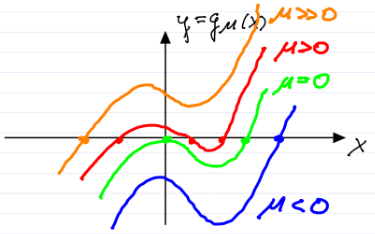
\includegraphics[width=0.4\textwidth]{figures/ch3/7gmu_roots.png}
		\caption{The functions $g_\mu $ for different values of $\mu $.}
		\label{fig:gmu_roots}
	\end{figure}
	By plotting $x$ as a function of $\mu $ such that $g_{\mu }(x)$ we get the \emph{bifurcation diagram} as shown in Fig. \ref{fig:gmu_bifurc}.
	\begin{figure}[h!]
		\centering
		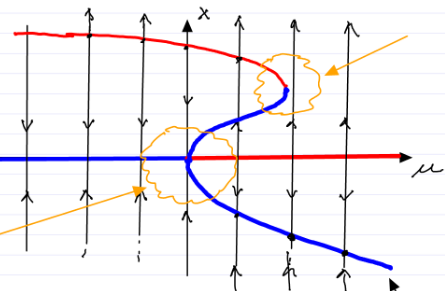
\includegraphics[width=0.6\textwidth]{figures/ch3/8gmu_bifurc.png}
		\caption{Bifurcation diagram for the 1-dimensional dynamical system. Red and blue demarcate if the fixed point at the given $(x, \mu)$ pair is stable (blue) or unstable (right). The arrow on the right points towards a \emph{fold bifurcation} and the arrow on the left towards a \emph{pitchfork bifurcation}.The curve is given by implicitly solving $g_{\mu}(x)=0$.}
		\label{fig:gmu_bifurc}
	\end{figure}

	The fold bifurcation (see caption of Fig. \ref{fig:gmu_bifurc}) is created by quartic (order 4) terms, which become more important away from the origin. The pitchfork bifurcation is already captured by the cubic truncation. We would like to know when the truncation captures the full dynamics correctly near the origin. Poincare showed that, in fact, the truncated system is topologically equivalent to the full system near the origin by using a change of coordinates to remove $\mathcal{O}(4)$ terms.

	\begin{enumerate}
		\item 		
	Let $x =y + h_4(y)= y+ay^4 + \mathcal{O}(y^5) $, which is near the identity near the origin, hence it is also invertible near the origin (by Implicit Function Theorem). Further, this preserves the ODE up to the $\mathcal{O}(3)$ terms.  
\item
	Plug in $x(t)$ and $y(t)$ and take the derivative with respect to time to get
	\begin{align}
		\dot{x} = \dot{y}(1+4ay^3 + \mathcal{O}(y^4)).
	\end{align}
\item 
Now use the ODE and find
\begin{align}
	\dot{x}=\mu x - x^3 +x^4 = \mu (y+ay^4)-(y+ay^4)^3 + (y-ay^4)^5 + \ldots.
\end{align}
\item
	Combine the previous two steps and calculate
\begin{align}
	\dot{y}= \left[1 + 4ay^3 + \mathcal{O}(y^4)\right]^{-1} \left[\mu y + a \mu y^4 - y^3+y^4 + \mathcal{O}(5)\right].	
\end{align}
At this point recall the von Neumann series (verify with Taylor expansion)
\begin{align}
	\frac{1}{1+z} = 1-z + \mathcal{O}(z^2);\quad 0 \leq |z| \ll 1.
\end{align}
Applying this to the left term in the formula for $\dot{y}$ yields
\begin{align}
	\left[1 + 4ay^3 + \mathcal{O}(y^4)\right]^{-1}=1 - 4ay^3 + \mathcal{O}(y^4). 
\end{align}
Therefore we find
\begin{align}
	\dot{y} &= \mu y - y^3 + y^4\underbrace{(-4a \mu  +a \mu +1)}_{ \textrm{choose }a  \textrm{ such that this }  =0} + \mathcal{O}(y^5),
\end{align}
the $a$ that fulfills this is $a=\frac{1}{3 \mu }$, using this we find
\begin{align}
	\boxed{
		\dot{y} = \mu y-y^3+\mathcal{O}(y^5).
	}
\end{align}
This transformation has removed the quartic terms from the equation.
\item
	Now we remove the $\mathcal{O}(y^5)$ terms similarly. First set 
	\begin{align}
		y = \xi + h_5(\xi) = \xi + b \xi^5 + \mathcal{O}(\xi^6)
	\end{align}
	and then continue as before, but with $y$ now playing the role of $x$ and $\xi$ playing the role of $y$.
\item The successive sequence of near identity coordinate changes turns out to converge usually. In general, it depends on the type of problem, sometimes resonant terms are not removeable and must stay as they are crucial to the dynamics. These terms depend on the linear part, for more see the book by Guckenheimer \& Holmes.
	\end{enumerate}
Thus 
\begin{align}
	\boxed{
\dot{x} = \mu x - x^3	
}
\end{align}
is the \emph{normal form} for the ODE for the study of bifurcations at the origin for $0 \leq \mu \ll 1$. It is topologically equivalent to the full system near $x=0$ and captures the pitchfork bifurcation.
\end{ex}

\section{Bifurcations}
A \emph{bifurcation} is a qualitative change in the dynamical system
\begin{align}
	\boxed{
		\dot{x} =f(x, \mu );\quad x \in \mathbb{R}^{n};\quad \mu \in \mathbb{R}^{p}.
	} \numberthis \label{eq4:astar}
	\end{align}
	Linear stability analysis led to reducing to the center manifold (depending on parameters). From there we moved to normal forms which enable the analysis of qualitative dynamics under varying parameters. 
	\begin{definition}[Local bifurcation]
		A \emph{local bifurcation} is a local near-equilibrium change in qualitative behavior. More precisely, a \emph{bifurcation} occurs in \eqref{eq4:astar} at $\mu = \mu _0$ near the fixed point $x=0$ if there exists no neighborhood of $x=0$ in which $\dot{x}=f(x, \mu _0)$ is topologically equivalent to \underline{all} systems $\dot{x} = f(x, \mu )$ for $\|\mu -\mu _0\|$ small enough.
	\end{definition}
	This idea of a bifurcation can be illustrated by a ``bifurcation" surface which separates the space of dynamical systems into components. Within each component the dynamical systems are topologically equivalent, however elements from separate components are not. This is sketched in Fig. \ref{fig:bif_surf_def}.
	\begin{figure}[h!]
		\centering
		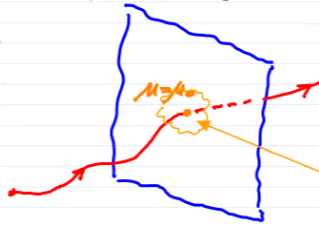
\includegraphics[width=0.5\textwidth]{figures/ch3/9bif_surf_def.png}
		\caption{Illustration of a bifurcation surface (blue). The near side of the surface is one component, and the far side the other. The red path is a family of dynamical systems $\{\dot{x} = f(x,\mu )\}_{\mu \in \mathbb{R}^{p}}$, going through the bifurcation point $\mu_0$. Around this point, a neighborhood as outlined in the definition is sketched in orange.}
		\label{fig:bif_surf_def}
	\end{figure}

We wish to understand what happens in the case that a given family of dynamical systems is nongeneric (atypical). For instance in the case that the family forms a tangency to the bifurcation surface, in which case a bifurcation does not take place, hence the family of dynamical systems is not general enough to capture all possible dynamics.

\begin{ex}[Nongeneric family of dynamical systems]
	In comparison to the family taken previously consider
	\begin{align}
		 \dot{x} = -a^2 x -x^3;\quad \mu =-a^2\leq 0.
	\end{align}
	For every $\mu $ which we consider, there is only one fixed point $x=0$ and it is stable for all values of $\mu $. However, we have unwittingly missed the full picture, as for $\mu >0$ there are three fixed points, two of which are unstable. This situation is shown in Fig. \ref{fig:nongen_ds}.
	\begin{figure}[h!]
		\centering
		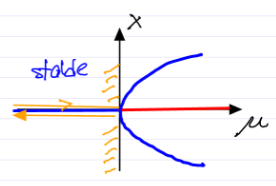
\includegraphics[width=0.4\textwidth]{figures/ch3/10nongen_ds.png}
		\caption{A nongeneric family of dynamical systems. We only see what happens to the left of the $x$-axis, and miss everything to the right, hence our family is tangent to the bifurcation surface.}
		\label{fig:nongen_ds}
	\end{figure}
\end{ex}

This idea of nongeneric families leads us to our next definition which is also depicted in Fig. \ref{fig:univ_unfold_def}.
\begin{definition}[Universal unfolding]
	A paramaterized family of dynamical systems crossing all nearby topological equivalence classes as the parameters vary is called a \emph{universal unfolding}.
\end{definition}
\begin{figure}[h!]
	\centering
	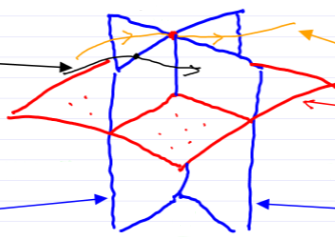
\includegraphics[width=0.45\textwidth]{figures/ch3/11univ_unfold_def.png}
	\caption{An example of universal unfolding (red) for the red bifurcation point which crosses the four topologically equivalent classes (components) created by the two bifurcation surfaces (blue). Furthermore, a nonuniversal unfolding is shown by the yellow 1-dimensional path at the top. Another universal unfolding in for the black bifurcation point, is shown by the 1-dimensional black family.}
	\label{fig:univ_unfold_def}
\end{figure}

\begin{definition}[Codimension of a bifurcation] The \emph{codimension of a bifurcation} is the minimum number of parameters required for a universal unfolding. Thus a more degenerate bifurcation requires a larger codimension.
\end{definition}

\section{Codimension 1 bifurcations}
